\documentclass[presentation]{beamer}
\usepackage[utf8]{inputenc}
\usepackage[T1]{fontenc}
\usepackage{fixltx2e}
\usepackage{textcomp}
\usepackage{hyperref}
\usepackage{siunitx}
\usepackage{booktabs}
\usepackage{movie15}
\usepackage{etex} 
\usepackage{pgfpages}
\usepackage{tikz}
\usepackage{will-beamer-baltimore} 
\usepackage{xcolor}
\tolerance=1000

\graphicspath{ 
  {figs/},
  {../TownsvillePoster/figs/},
  {../LarimTalk2010/movies/},   
  {../Poland2012/figs/},   
}

\newcommand\backskip{\vspace*{-\baselineskip}}
\newcommand\backsmallskip{\vspace*{-\smallskipamount}}
\newcommand\backmedskip{\vspace*{-\medskipamount}}
\newcommand\backbigskip{\vspace*{-\bigskipamount}}

\setkeys{Gin}{width=\linewidth, height=0.8\textheight, keepaspectratio=true}

% \setbeameroption{show notes}

% \renewcommand\baselinestretch{1.2}

\title{Dynamics of the Orion Nebula: ISM}
\author{\textit{William J. Henney}}
\date[Baltimore 2013]{October 2013 \(\cdot\) STScI, Baltimore}
\institute[CRyA, UNAM]
{
  \structure{Centro de Radioastronomía y Astrofísica\\
  UNAM, Morelia, México}
}

\hypersetup{
  pdfkeywords={Orion Nebula, Astrophysics, Dynamics},
  pdfsubject={},
  pdfcreator={Lovingly hand-crafted by the author using pdflatex and beamer}
}


\AtBeginSection[]
{
  \begin{frame}<beamer>
    \frametitle{Coming up next \dots}
    \tableofcontents[
    sectionstyle=show/shaded,
    currentsubsection, 
    hideothersubsections
    ]
  \end{frame}
}



\begin{document}

\maketitle

\begin{frame}
\frametitle{Principal collaborators}

\begin{block}{CRyA-UNAM, Morelia, Mexico}
\begin{description}
\item[\small HD] \textit{Jane Arthur}
\item[\small Turbulence] \textit{Enrique Vázquez-Semadeni}
\item[\small Students] \textit{Sac-Nicté Serrano Medina}
\item \textit{A. Jorge Tarango Yong}
\item \textit{Luis Ángel Gutierrez Soto} 
\end{description}
\end{block}

\begin{block}{Elsewhere}
  \begin{description}
  \item[\small MHD] \textit{Fabio de Colle} (ICN-UNAM, Mexico)
  \item[\small Radiation] \textit{Garrelt Mellema} (Stockholm Observatory, Sweden)
  \item[\small Observations] \textit{María Teresa García-Díaz} (IA-UNAM, Ensenada, Mexico)
  \item \textit{Bob O'Dell} (Vanderbilt, USA)
  \item \textit{Bob Rubin} \textbf{[\textdagger{} 2013-03-03]} (NASA-AMES/Orion Enterprises)
  \end{description}
\end{block}

\end{frame}

\begin{frame}<beamer>
  \frametitle{Dynamics of the Orion Nebula}
  \tableofcontents[hidesubsections]
\end{frame}

\section{Observational diagnostics of Orion Nebula dynamics}
\label{sec:obs}

\begin{frame}
  \frametitle{How can we observe gas motions in the nebula?}
  \begin{block}{Emission line spectroscopy}
    \begin{itemize}
    \item Motions along line of sight only
    \item Affected by thermal broadening
    \end{itemize}
  \end{block}

  \begin{block}{Proper motions}
    \begin{itemize}
    \item Motions in plane of sky
    \item Gives pattern speed, not gas velocity
      \begin{itemize}
      \item \(\Rightarrow\) non-steady motions only
      \end{itemize}
    \item Requires spatially sharp emission features and relatively high velocities
      \begin{itemize}
      \item \(\Rightarrow\) best suited to jets and other outfows
      \end{itemize}
    \end{itemize}
  \end{block}
  
  \begin{block}{Test particles}
    \begin{itemize}
    \item Use of stellar bowshocks to probe the nebular flow
    \end{itemize}
  \end{block}

  \end{frame}

\subsection{Radial velocities}
\begin{frame}
  \frametitle{Slicing the velocity cubes}
  \foreach \y [count=\x] in {52,53,...,85} {%
    \only<\x>{\includegraphics[page=\y, trim=0 30 0 75,clip]{oldtalks/windsor-talk.pdf}}%
  }%
\end{frame}

\subsection{Proper motions}

\begin{frame}
  \frametitle{Non-steady motions of jet knots}
  \hfill
  \includegraphics[height=0.8\textheight]{LL2-Will-Crop-Annotate}
  \hfill
  \includegraphics[height=0.8\textheight]{LL2-propermotions3.pdf}
  \hfill\null
\end{frame}

\begin{frame}
  \frametitle{Jets are everywhere in Orion}
  \makebox[0pt][l]{\hspace*{0.3\textwidth}\includegraphics{OH2008-fig5}}%
  \only<2->{\makebox[0pt][l]{\includegraphics[width=0.5\textwidth]{bob-arrows6}}}%
  \only<3>{\includegraphics[width=0.5\textwidth]{OH2008-fig7}}
\end{frame}


\subsection{Test particles}

\begin{frame}
  \frametitle{Stationary bowshocks as probes of the nebular flow}
  \includegraphics{LL1-schematic}
\end{frame}

\begin{frame}
  \frametitle{More bowshocks}
  \renewcommand\arraystretch{0}
  \setlength\tabcolsep{0pt}
  \begin{tabular}{l}
    \includegraphics[height=0.8\textheight]{north-west-field-combined}\\
  \end{tabular}%
  \begin{tabular}{l}
    \includegraphics[height=0.266\textheight]{LL266-558-15x15arcsec-annot}\\
    \includegraphics[height=0.266\textheight]{Proplyd-Bow2-10x10arcsec-annot}\\
    \includegraphics[height=0.266\textheight]{LL6-60x60arcsec-annot}\\
  \end{tabular}
\end{frame}

\begin{frame}
  \frametitle{Two-shock stationary flow pattern}
  \centering\includegraphics[width=\textwidth]{LL-outer-inner}
\end{frame}

\section{Physical ingredients for dynamic models}

\subsection{Governing equations}
\begin{frame}
  \frametitle{Governing equations}
  \begin{block}{Euler equations}
    Conservation of mass, \alert{momentum}, energy
  \end{block}
  \begin{block}{Ionization balance}
    Global and local ionization parameter
  \end{block}
  \begin{block}{Radiative transfer}
    \alert{Ionizing radiation}, non-ionizing radiation, X-rays
  \end{block}
  \begin{block}{Want more details?}
    See \href{http://adsabs.harvard.edu/abs/2007dmsf.book..103H}{Henney \texttt{2007dmsf.book..103H}}
  \end{block}
\end{frame}



\begin{frame}
  \frametitle{Euler equations}
  \begin{centering}
    \includegraphics[width=.8\linewidth]{EulerEquations.jpg}\par
  \note{
    \[
    \frac{d}{dt} ( \rho \VEC{u} ) + \VEC{\grad} ( P + \rho u^2 ) = \rho \VEC{a} 
    \]
  }
  \note{ There is also an energy equation, which is important in some
    circumstances.  But in the ionized gas, it can usually be replaced
    by the isothermal assumption.  }
  \end{centering}
\end{frame}

\subsection{Ionization balance}

\begin{frame}
  \frametitle{Ionization balance}
  \only<1>{%
  \begin{block}{Local ionization parameter}
    Dimensionless ratio of ionizing photon density to gas particle density
    \[
    \Upsilon = \frac{F_{\mathrm{ion}}}{c n} 
    \]
    In static equilibrium, the Hydrogen ionization fraction \(x\)
    satisifies 
    \[
    \frac{x^2}{1 - x} \simeq \num{3e5}\, \Upsilon
    \]
  \end{block}}
  \only<2>{%
  \begin{block}{Global ionization parameter}
    For static, ionization-bounded region:
    \[
    \langle\Upsilon\rangle \simeq 0.006 
    \left(  
      \frac{\langle n\rangle_{\mathrm{rms}}}{\SI{e3}{cm^{-3}}}
    \right)^{1/3} 
    \left(  
      \frac{Q_{\mathrm{H}}}{\SI{e49}{s^{-1}}} 
    \right)^{1/3} 
    \]
    \begin{itemize}
    \item For a given dust-gas ratio, dust opacity is more important at high \(\langle\Upsilon\rangle\)
    \item Advective (flow) terms are globally more important in the ionization
      and heating/cooling balance for low \(\langle\Upsilon\rangle\)
    \end{itemize}
  \end{block}}
  \only<3>{%
  \begin{block}{Heavy-element ionization}
    \bigskip
    \begin{centering}
      \includegraphics[height=0.7\textheight]{oldtalks/TFE06/lineplot.pdf}\par
    \end{centering}
  \end{block}}
\end{frame}


\begin{frame}[c]
  \frametitle{Ionization structure in the Orion Nebula}
  \setkeys{Gin}{height=0.8\textheight, keepaspectratio=true}
  \begin{centering}
    \only<1>{\includegraphics{oldtalks/TFE06/All_quart}}%
    \only<2>{\includegraphics{oldtalks/TFE06/All_quart_hilight}}%
    \par
  \end{centering}
\end{frame}

\begin{frame}
  \frametitle{Complex ionization structure in the heart of the nebula}
  \setkeys{Gin}{height=0.8\textheight, keepaspectratio=true}
  \begin{centering}
    \only<1>{\includegraphics{oldtalks/TFE06/talk_image_658+656+502}}%
    \only<2>{\includegraphics{oldtalks/TFE06/talk_image_658+673+631}}%
    % \only<1,7>{\includegraphics{oldtalks/TFE06/talk_image_658+656+502}}%
    % \only<2,6>{\includegraphics{oldtalks/TFE06/talk_image_658+673+631}}%
    % \only<3>{\includegraphics{oldtalks/TFE06/talk_image_658+673+631_labels}}%
    % \only<4>{\includegraphics{oldtalks/TFE06/talk_image_658+673+631_oneray}}%
    % \only<5>{\includegraphics{oldtalks/TFE06/talk_image_658+673+631_bothrays}}%
    \par
  \end{centering}
\end{frame}

\subsection{Radiative transfer}

\begin{frame}
  \frametitle{Radiative transfer}
  \begin{block}{Ionizing radiation}
    \begin{itemize}
    \item All absorbed in \hii{} region (or ionization front)
    \item Higher density gas absorbs more efficiently (per unit mass)
    \end{itemize}
  \end{block}
  \begin{block}{FUV/optical radiation}
    Some absorbed in \hii{} region but mainly in near PDR (PAH excitation)
  \end{block}
  \begin{block}{X rays}
    \begin{itemize}
    \item Produced by T Tauri chromospheres: \(\sim 1~L_\odot\)
    \item Produced by base of O~star wind: \(\sim 1~L_\odot\)
    \item Produced by shocked stellar wind bubble: \(\sim 0.01~L_\odot\)
    \item Absorbed in far PDR and molecular gas
    \end{itemize} 
  \end{block}
\end{frame}

\subsection{Body forces}

\begin{frame}
  \frametitle{Body forces}
  \begin{block}{Gravity}
    Only important in the molecular gas
  \end{block}
  \begin{block}{Radiation pressure}
    \begin{itemize}
    \item Trapped resonance lines (e.g., Lyman \(\upalpha\))
    \item Ionizing radiation momentum acting directly on gas
      \begin{itemize}
      \item Only important for \emph{very} high ionization parameter, \(\Upsilon\)
      \end{itemize}
    \item \alert{Lower energy radiation absorbed by dust}
      \begin{itemize}
      \item Important for high ionization parameter, \(\Upsilon\)
      \item Collisionally coupled to gas
      \end{itemize}
    \end{itemize}
  \end{block}
\end{frame}

\subsection{Magnetic fields}


\begin{frame}
  \frametitle{Magnetic fields}
  \begin{block}{\emph{No time today!} \quad But please see \dots}
    \begin{columns}
      \column{0.6\linewidth}
      \includegraphics{poland-figs/Masthead-Henney-2009.png}\par
      \bigskip 
      \includegraphics{poland-figs/Masthead-Arthur-2011.png}\par
      \column{0.4\linewidth}
      \includegraphics{poland-figs/Streamers}\par
      \bigskip 
      \includegraphics{poland-figs/Globule-Structure-New}\par
    \end{columns}
  \end{block}
\end{frame}

\section{Building blocks for the internal dynamics}

\subsection{Thermal pressure gradients}

\begin{frame}
  \frametitle{Thermal pressure gradients \dots}
  \only<1>{%
  \begin{block}{\dots drive the non-steady global expansion of the \hii{} region}
    \begin{centering}
      \includegraphics[trim=0 300 0 150, clip, height=0.6\textheight]{poland-figs/Ipad-Sketch-HII-Expansion}\par
    \end{centering}
    Note that the neutral gas expands faster than the ionized gas.
  \end{block}}
  \only<2>{%
  \begin{block}{\dots drive steady-state photoevaporation flows}
    From globules, filaments, escarpments, proplyds, etc\par
    \begin{centering}
      \includegraphics[height=0.6\textheight]{poland-figs/Ipad-Sketch-Globule}\par
    \end{centering}
    Here, the ionized gas moves fastest.
  \end{block}}
\end{frame}

\begin{frame}[squeeze, shrink=5]
  \frametitle{Steady flow down a pressure gradient}
  \begin{block}{Steady-state continuity equation}
    \[
    \rho u r^k = \text{constant} \quad 
    k = \left\{\scriptstyle
      \begin{array}{ll}
        0 & \text{ (plane)}\\
        1 & \text{ (cylindrical)}\\
        2 & \text{ (spherical)}
      \end{array}
    \right.
    \]
  \end{block}
  \begin{block}{Isothermal Bernoulli equation}
    \[
    \frac12 u^2 + c_0^2 \ln \rho  + \Phi = \text{constant along a streamline}
    \]
  \end{block}
  \begin{block}{Condition for acceleration of a diverging flow}
    \[
    \frac{du}{dr} > 0  \quad \text{if} \quad u > c_0 \quad \text{and} \quad
    k > 0
    \]
  \end{block}
\end{frame}



\subsection{Steady-state photoevaporation flows}

\begin{frame}
  \frametitle{Corrugated ionization fronts}
  \foreach \y [count=\x] in {41,42,43} {%
    \only<\x>{\includegraphics[page=\y, trim=0 23 0 68,clip]{oldtalks/windsor-talk.pdf}}%
  }%
\end{frame}

\newcommand\missingmovietext{
  \begin{center}
    \bfseries\ttfamily
    This PDF viewer does not support embedded videos
    \par \bigskip
    To view the movie, please open the PDF file in \textit{Adobe Reader}
    
  \end{center}
  }

{
  \usebackgroundtemplate{
    \parbox[c][\paperheight][c]{\paperwidth}{\missingmovietext}
  }
\begin{frame}
  \def\DIR{/Users/will/Dropbox/Presentations/HoustonTalk2011/movies} 
  \frametitle{Photoevaporation of isolated globules   \quad \Ref{\small Henney et al. (2009)}}
  \begin{columns}
    \column{0.5\linewidth}
    \includemovie[label=glob-s80-255-side, autoplay, autopause, repeat, controls]
    {\linewidth}{0.498\linewidth}{\DIR/rgb-NHO-s80-255-evo+350+350.avi}\\
    \bigskip
    \includemovie[label=glob-s80-255-top, autoplay, autopause, repeat, controls]
    {\linewidth}{0.498\linewidth}{\DIR/rgb-NHO-s80-255-evo+010+080.avi}
    \column{0.5\linewidth}
    \includemovie[label=glob-s80-127-side, autoplay, autopause, repeat, controls]
    {\linewidth}{0.498\linewidth}{\DIR/rgb-NHO-s80-127m-evo+350+350.avi}\\
    \bigskip
    \includemovie[label=glob-s80-127-top, autoplay, autopause, repeat, controls]
    {\linewidth}{0.498\linewidth}{\DIR/rgb-NHO-s80-127m-evo+010+080.avi}
  \end{columns}
  \bigskip
  \centerline{\color{red}{[N\,II]}\quad
    \color{green}{H\(\upalpha\)}\quad
    \color{blue}{[O\,III]}}
\end{frame}
}

\subsection{Winds, shocks, shells}
{
  \usebackgroundtemplate{
     {\centering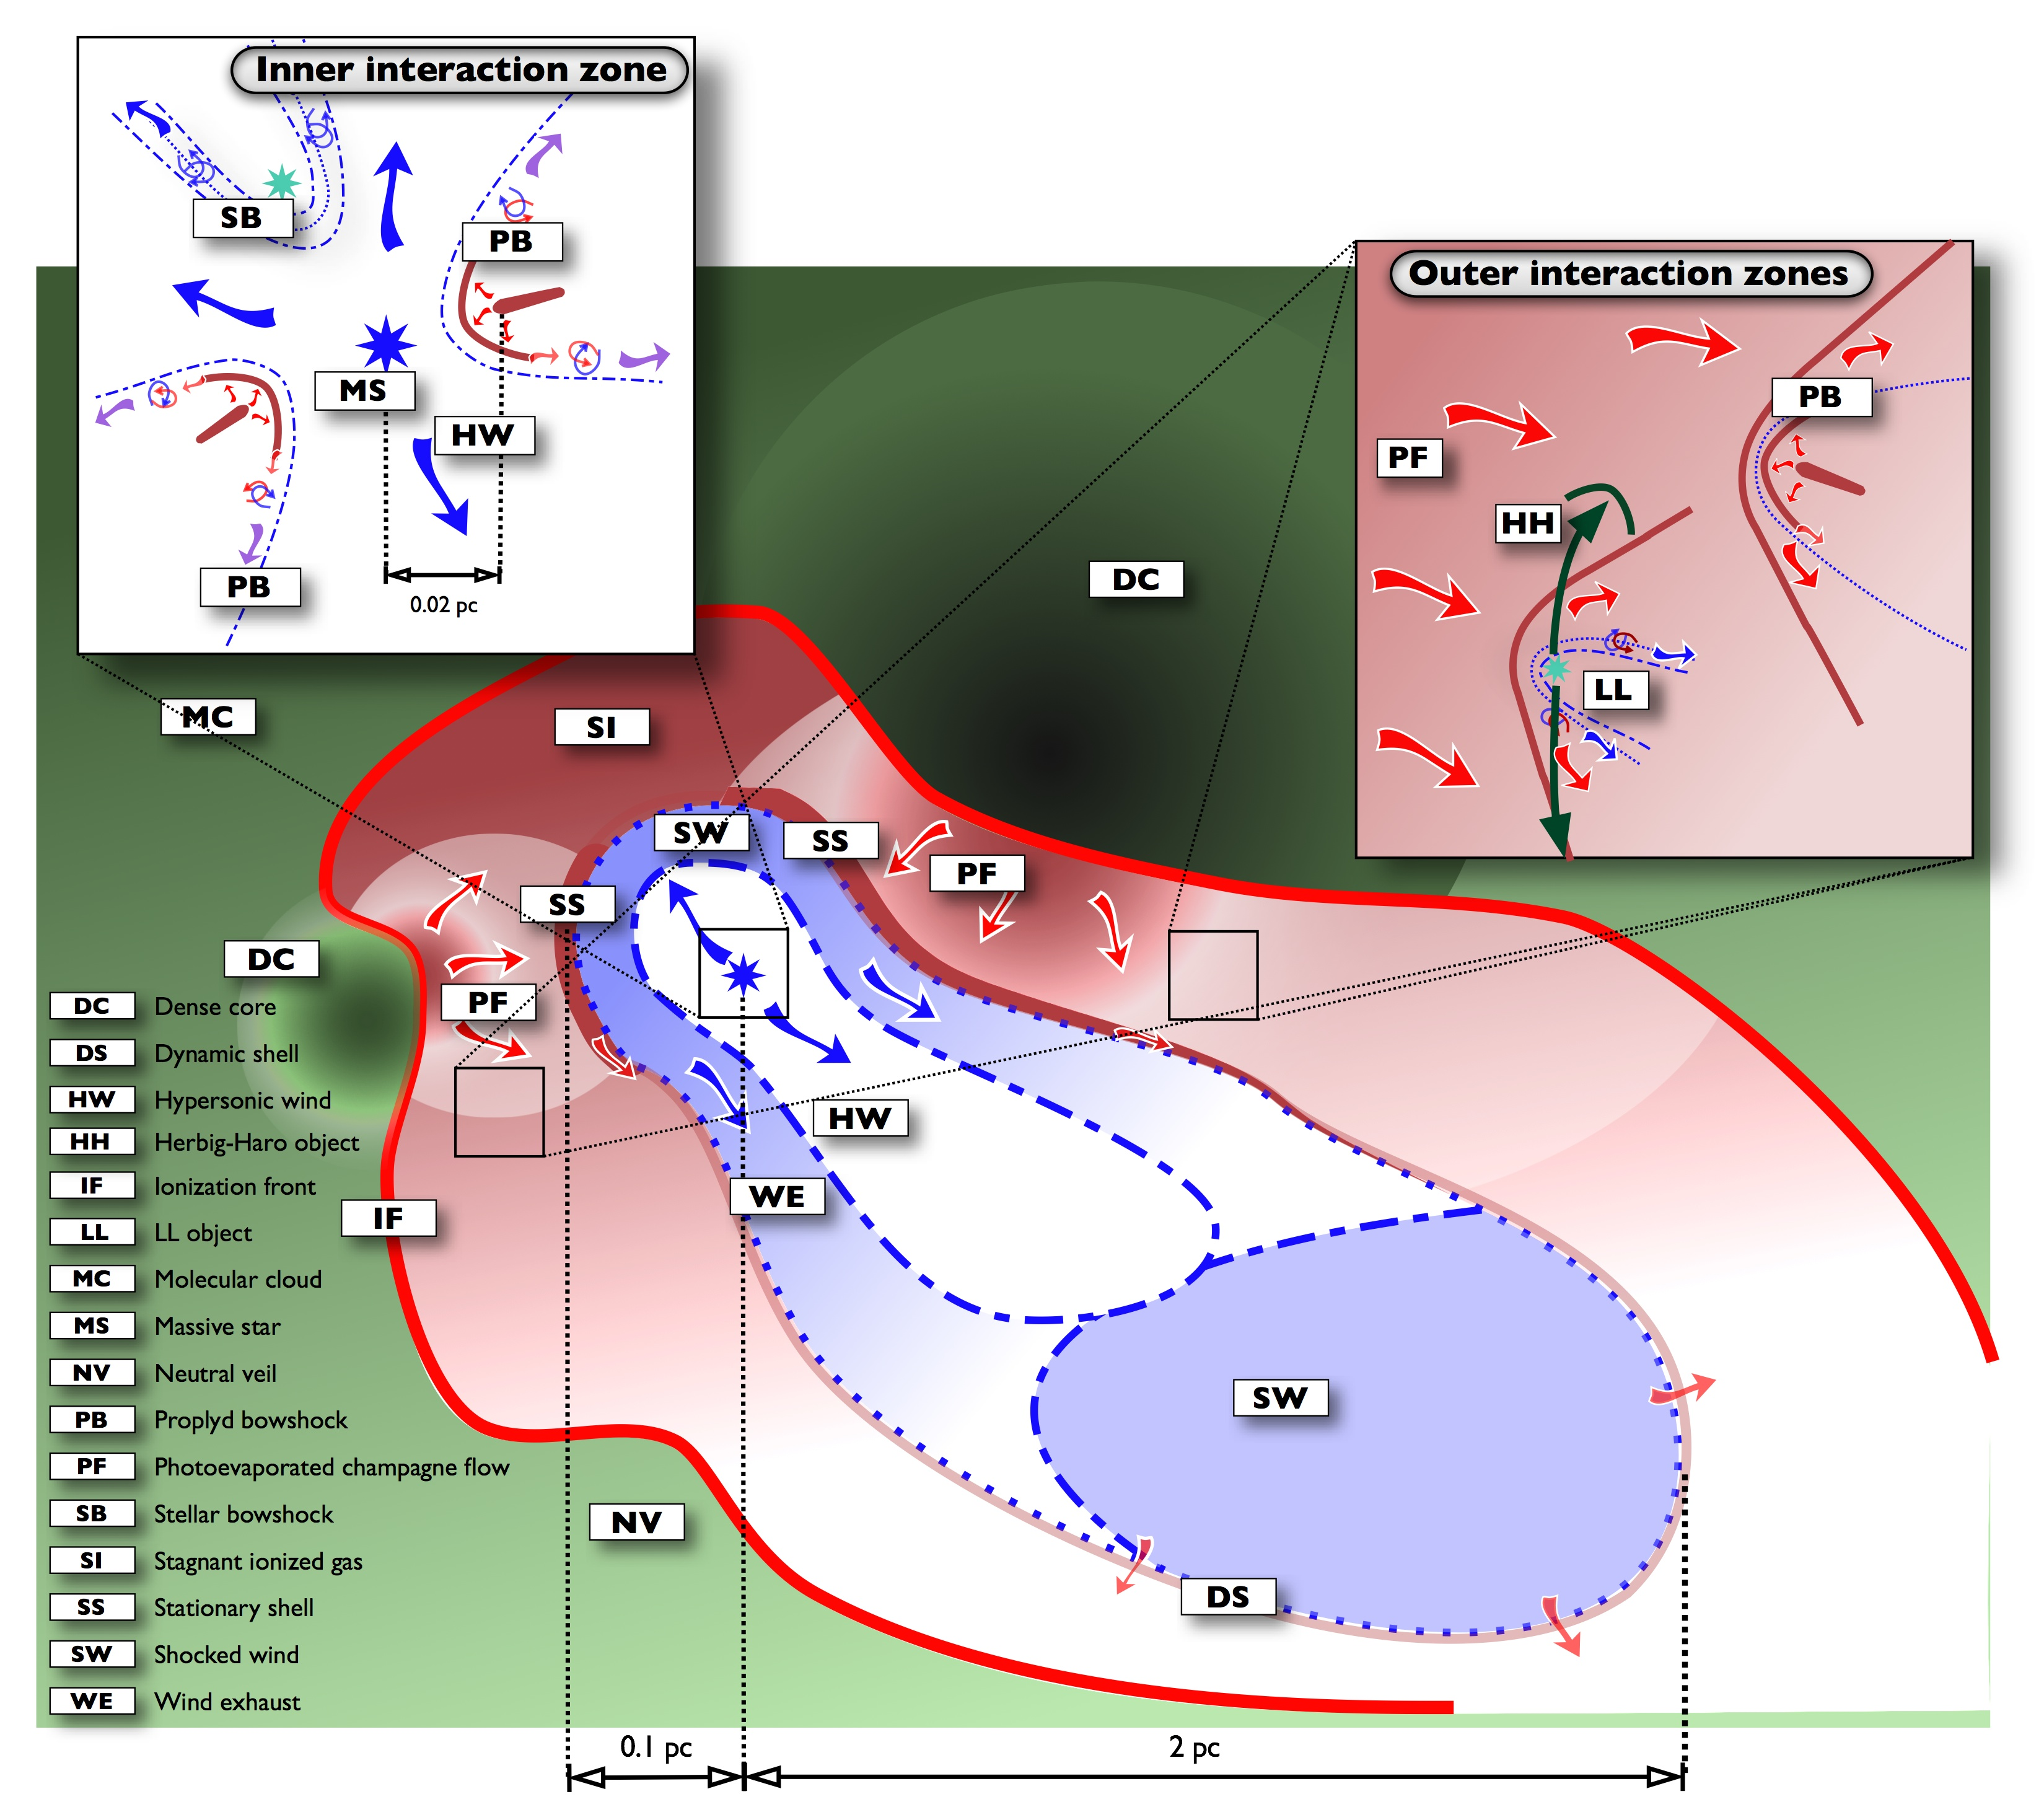
\includegraphics[height=0.93\paperheight]{wind-geometry-extended}}
  }
\begin{frame}
  \frametitle{\hspace*{0.5\textwidth}Winds, shocks, shells}
%  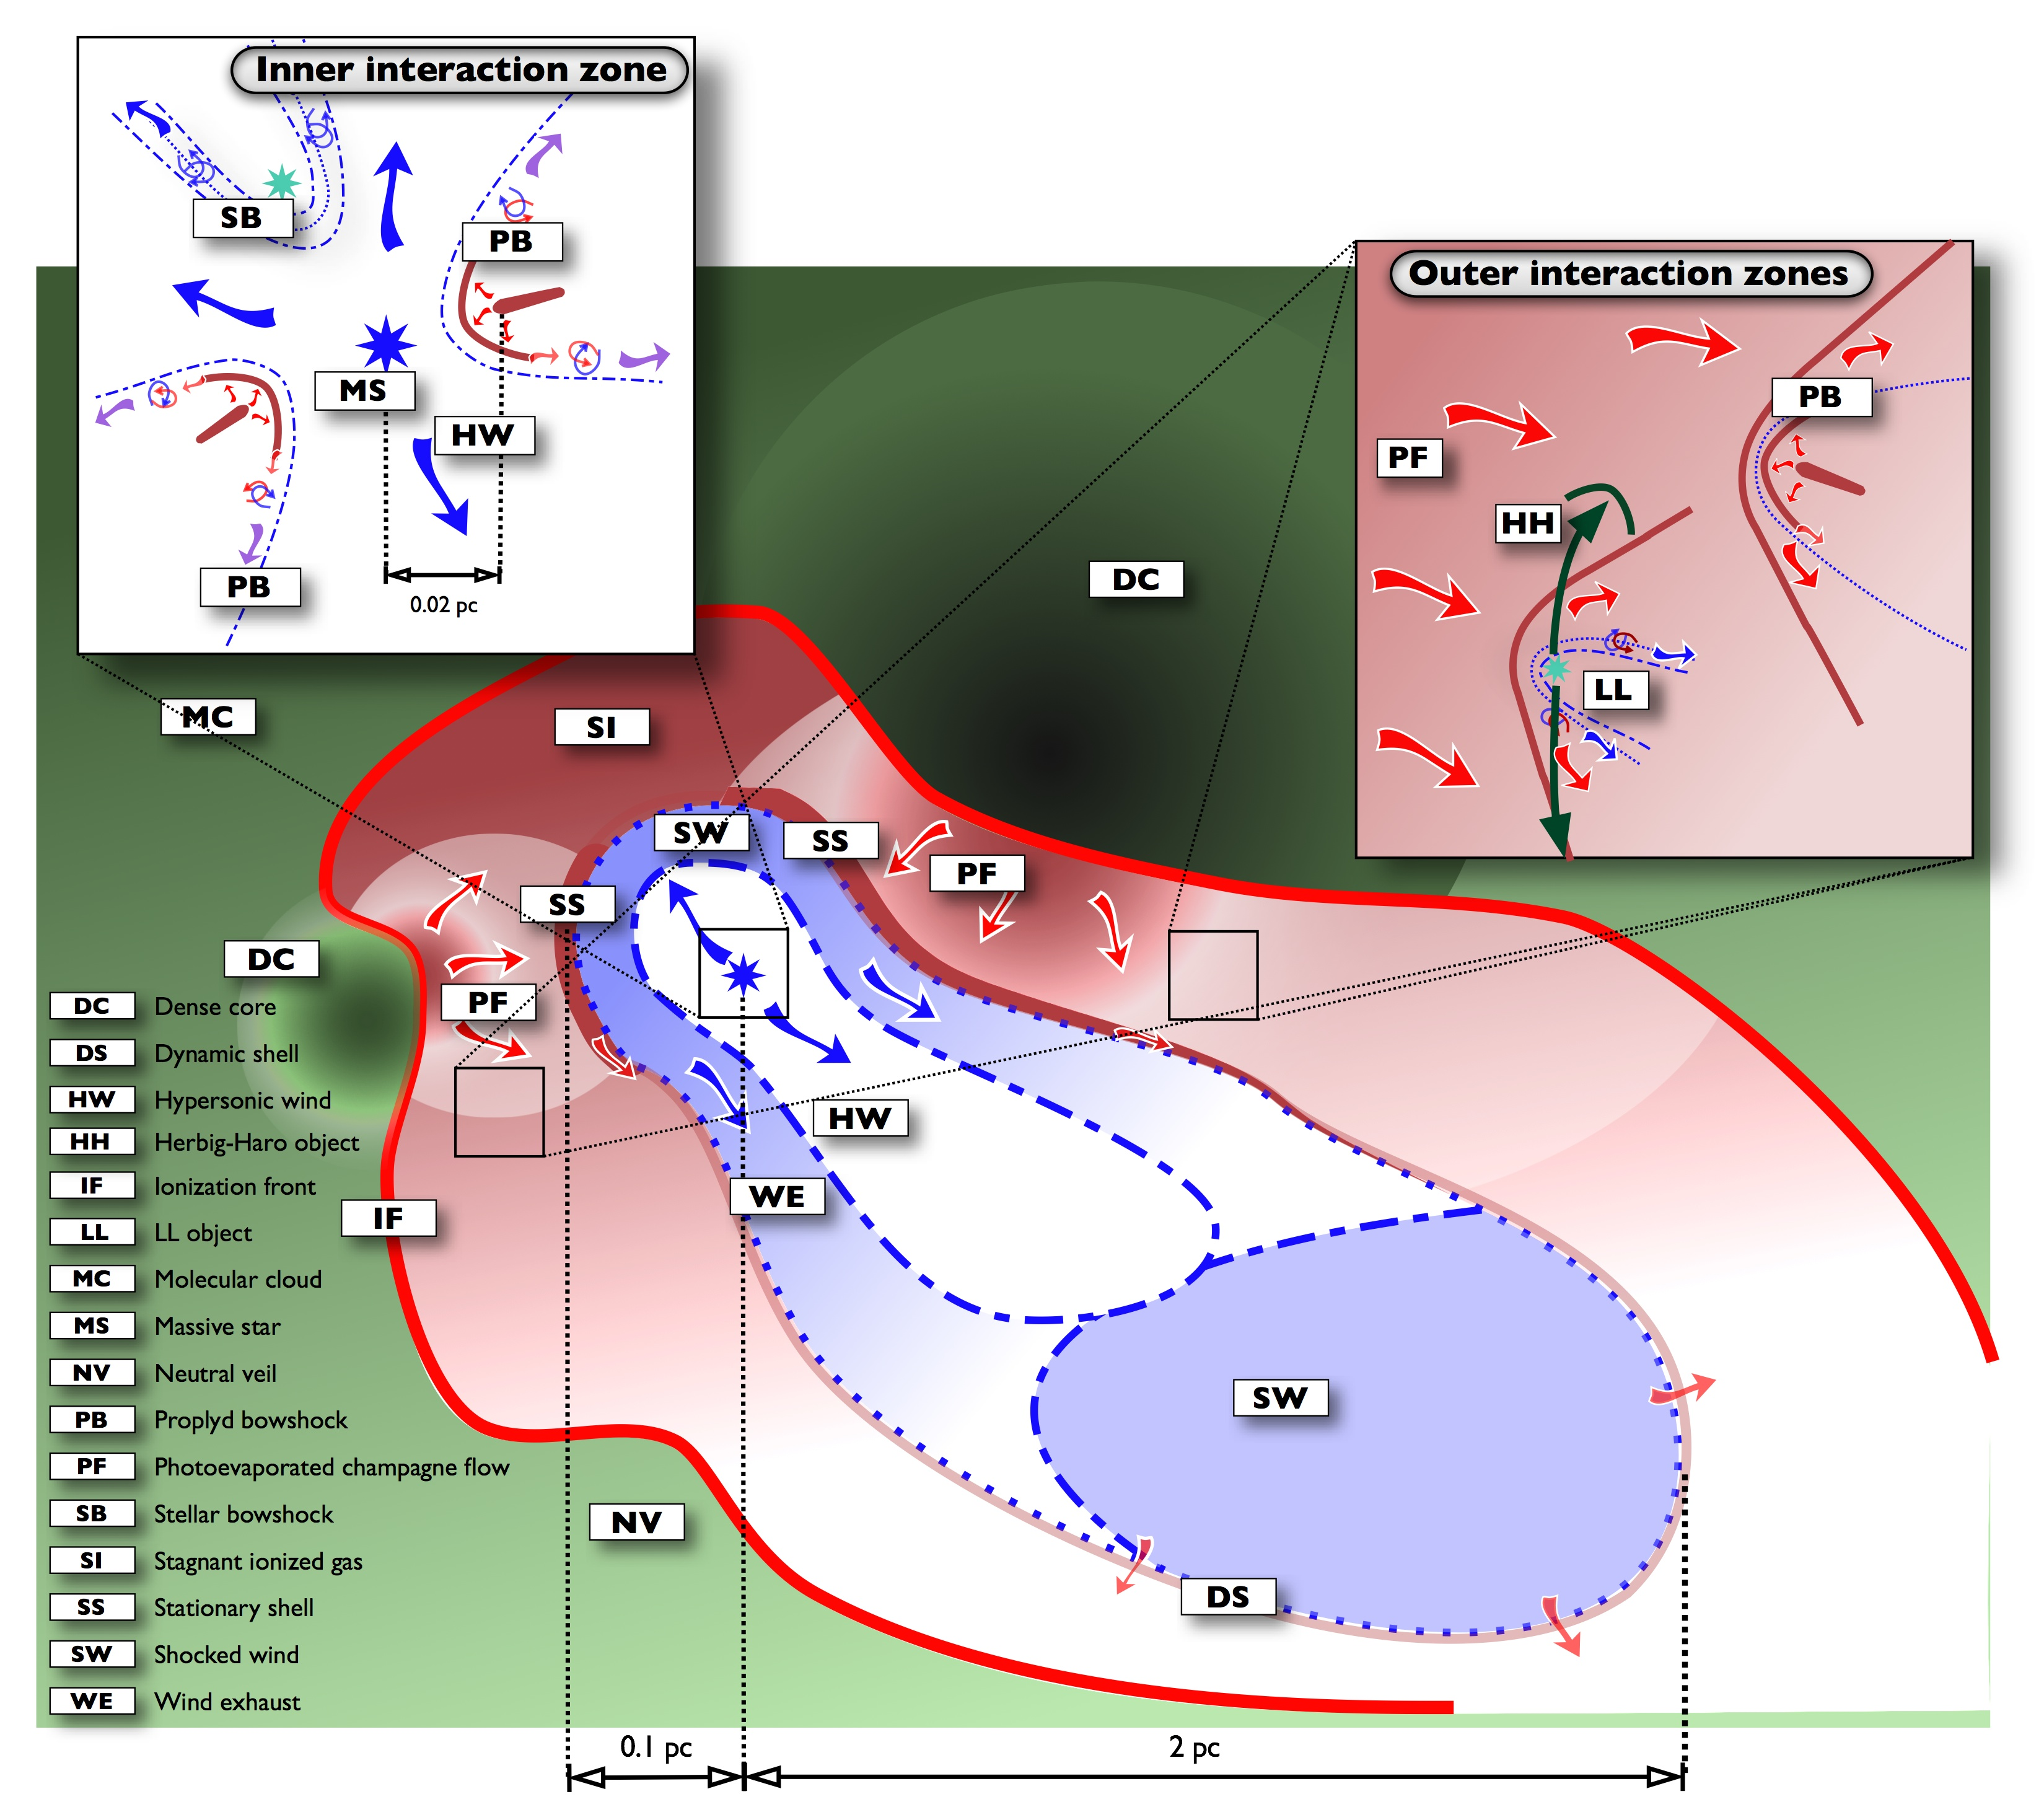
\includegraphics[width=\textwidth]{wind-geometry-extended}
  % \begin{block}{\emph{No time today!} }
  %   \includegraphics{poland-figs/Ipad-Sketch-Shocks}
  % \end{block}
\end{frame}
}

\section{Application of \hii{} region models to Orion}

\begin{frame}
  \frametitle{Application of \hii{} region models to Orion}
  \begin{block}{Simple models}
    \begin{itemize}
    \item \alert{Analytic calculation} or numerical simulations
    \item High degree of symmetry (1D plane or \alert{2D cylindical})
    \item Possibility to include realistic microphysics
    \end{itemize}
  \end{block}

  \begin{block}{Turbulent models}
    \begin{itemize}
    \item Numerical simulations only
    \item Fully 3D, no particular symmetry imposed
    \item \alert{But \dots}
      \begin{itemize}
      \item Simplified microphysics, {\scriptsize albeit a big
          improvement on the competition!}
      \item Uncertain initial conditions
      \end{itemize}
    \end{itemize}
  \end{block}

\end{frame}


\subsection{Simple models}

\begin{frame}
  \frametitle{Steady flow from a plane ionization front}
  \foreach \y [count=\x] in {35,36,37,38} {%
    \only<\x>{\includegraphics[page=\y, trim=0 30 0 75, clip]{oldtalks/windsor-talk.pdf}}%
  }%
\end{frame}




\subsection{Turbulent models}

\newlength\maxheight
\setlength\maxheight{0.8\textheight}
\newlength\moviewidth
\setlength\moviewidth{0.7\textwidth}

\begin{frame}
\frametitle{Turbulent models: initial conditions}
\includegraphics{poland-figs/rgb-CPF-initial}
\end{frame}

\begin{frame}[shrink=5]
\frametitle{Turbulent models: state of play}
\begin{block}{Physics we have}
  \begin{itemize}
  \item 3D time-dependent, hydrodynamics
  \item Approximate radiative transfer
  \item Microphysics:
    \begin{itemize}
    \item good for ionized gas
    \item fair for PDR
    \item poor for molecular gas
    \end{itemize}
  \item {}[Ideal magnetohydrodynamics]
  \end{itemize}
\end{block}
\begin{block}{Physics we lack}
  \begin{itemize}
  \item Stellar winds
  \item Radiation pressure
  \item Diffuse field
  \item Self-gravity
  \item {\footnotesize Better microphysics, better radiative transfer,
    \scriptsize multifluids, non-ideal MHD, \tiny \(\upkappa\)-distributions, etc \dots}
  \end{itemize}
\end{block}
\end{frame}

\begin{frame}[plain]%%
  \newlength\figwidth
  \setlength\figwidth{0.33\textwidth}
  \renewcommand\arraystretch{0.0}
  \setlength\tabcolsep{0pt}
  \graphicspath{
    {poland-figs/movie-stills/O-Star-512-PDR-2012/},
    }
  \begin{tabular}{lll}
    \includegraphics[width=\figwidth]{01-Opening-Titles}
    & 
    \includegraphics[width=\figwidth]{02-Model-Parameters}
    & 
    \includegraphics[width=\figwidth]{03-Color-Scheme}
    % & 
    % \includegraphics[width=\figwidth]{04-Evolution-Start}
    \\
    \includegraphics[width=\figwidth]{05-Evolution-Mid}
    & 
    \includegraphics[width=\figwidth]{06-Evolution-End}
    & 
    \includegraphics[width=\figwidth]{07-Detail-View}
    % & 
    % \includegraphics[width=\figwidth]{08-Swimming-Sisters} 
    \\
    % \includegraphics[width=\figwidth]{09-Long-Wav-Color-Scheme}
    % & 
    \includegraphics[width=\figwidth]{10-Long-Wav-Mid}
    & 
    \includegraphics[width=\figwidth]{11-Long-Wav-End}
    & 
    \includegraphics[width=\figwidth]{12-Simulations-Credit}
\end{tabular}

\end{frame}


\begin{frame}
  \frametitle{Turbulent models: results}
  \begin{columns}
    \column{0.6\linewidth}
    \begin{itemize}
    \item Many morphological features of observed \hii{} regions are
      reproduced naturally
      \begin{itemize}
      \item Due to existing density structure in the
        turbulent molecular cloud, combined with fragmentation induced
        by interaction with the ionized gas
      \end{itemize}
    \item Velocity dispersions of order the sound speed are
      maintained in the ionized gas during the entire evolution
    \item The highest pressure neutral/molecular gas is driven to
      equipartition between thermal, magnetic, and turbulent energies
    \item Lower pressure gas bifurcates into zones dominated by one or
      the other
    \end{itemize}
    \column{0.4\linewidth}
    \includegraphics{poland-figs/comparison3_vs_t_Ostar}%
  \end{columns}
\end{frame}

\begin{frame}
  \frametitle{Turbulent models: more results}
  \begin{columns}
    \column{0.5\linewidth}
    \includegraphics{poland-figs/mhd-pressures-rgb-Ostar-et-0200-pram-pmag}
    \column{0.5\linewidth}
    \includegraphics{poland-figs/mhd-pressures-rgb-Ostar-et-0200-n-B}
  \end{columns}
\end{frame}

% {
%   \usebackgroundtemplate{
%     \parbox[c][\paperheight][c]{\paperwidth}{\missingmovietext}
%   }
\begin{frame}[plain]%%
\hspace*{-1ex}\includemovie[label=new-movie, autoplay, autopause, controls, repeat=1]
{1.27968\paperheight}{0.96\paperheight}{poland-figs/O-Star-512-PDR-2012.mov}
\end{frame}
% }



\end{document}
